
\documentclass[12pt, oneside]{extbook} % the document type needs to be change
\usepackage{geometry}
\usepackage{listings}
\usepackage{graphicx}
\usepackage[utf8]{inputenc}
\usepackage[T1]{fontenc}
\usepackage[italian]{babel}

\geometry{
    top = 1.5cm,
    bottom = 1.5cm,
    left = 2cm,
    right=2cm,
}

\begin{document}
\chapter{DNS Security}

\section{Introduzione}
DNS è uno dei più vecchi e fondamentali componenti dell'Internet, ovviamente anche questo non è stato progettato con la sicurezza in mente.
\\La rete si è evoluta, quindi è cominciata una discussione per renderlo più sicuro, mediante DNSSEC.
\\Sappiamo che se un client vuole connettersi ad un sito, deve conoscere l'IP del sito e quindi manda una richiesta UDP, dove la chiave è tipicamente un nome, si ottengono uno o più record in base ai tipi di risorsa.
\\Una delle risorse più importanti è A, che è proprio un indirizzo IP.
\\Se scendiamo nel dettaglio, abbiamo una richiesta ed una risposta, DNS è un protocollo binario, dove si richiede ad esempio il record A di un nome associato ad una chiave "sito.com", ma questo dipende appunto dalla richiesta che si fa, anche la risposta quindi dipenderà dal record.
\\DNS è un protocollo ed un DB chiave:valore distribuito, le chiavi consistono in nome, chiave e classe.
\\Lo spazio dei nomi è gerarchico, avremo quindi delle zone per cui c'è un server autoritativo che mantiene i record DNS per quella zona.
\\Un DNS resolver chiederà ad un server autoritativo apposito per ottenere l'informazione richiesta, tipicamente il mio DNS resolver non è ricorsivo, ma fa una richiesta che viene risolta in maniera ricorsiva chiedendo ai diversi server autoritativi.
\\Si segue la gerarchia:\\
\begin{figure}[h!]
    \centering
    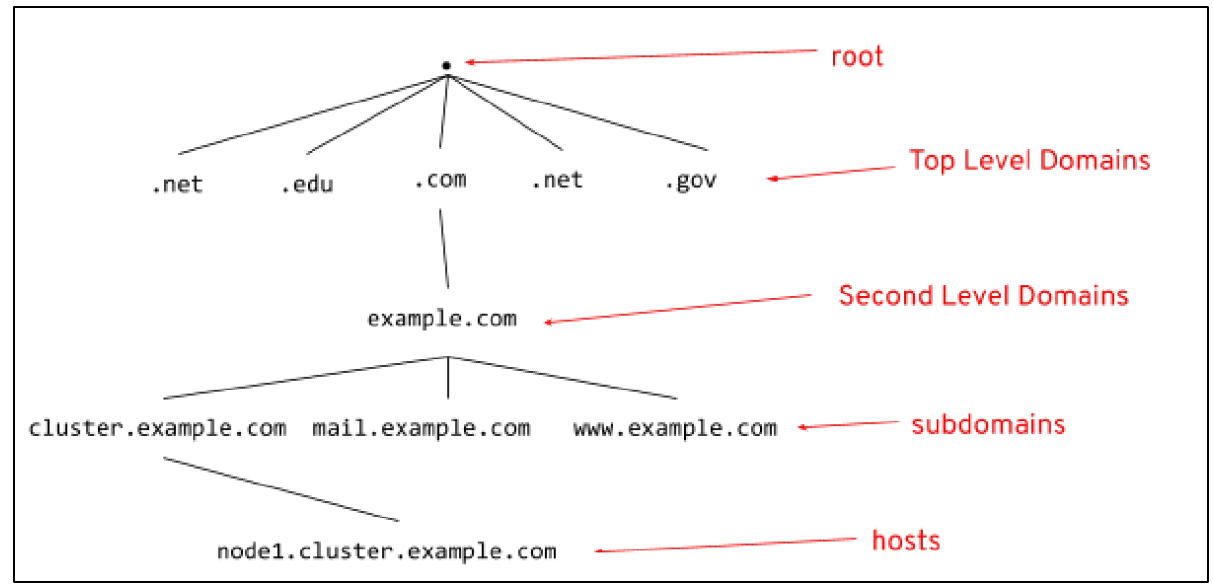
\includegraphics[scale=0.5]{../../immagini/dns_hier}
\end{figure}\\\\
possiamo anche avere sotto-domini, e questo processo può essere ripetuto, avendo quindi dei sotto-domini per i sotto-domini.

\subsection{Risoluzione di una query}
Quando si fa una query ad un resolver, se questa è già in cache si manda direttamente in risposta, ci sono 13 server di root e per ogni top level domain c'è almeno un authoritative nameserver.
\\Partendo dalla root, vogliamo risolvere "example.com":
\begin{itemize}
	\item il root server da l'IP del TLD per example.com
	\item si prosegue così finché non si arriva al server che può rispondere alla query richiesta
\end{itemize}

Ci sono 4 server contattati durante una query:
\begin{itemize}
	\item name server autoritativo che fa il lookup ricorsivo
	\item Root name server, ha tutti i name server per i TLD
	\item TLD nameserver 
	\item authoritative nameserver
\end{itemize}
Quindi, per poter ottenere un dominio, facciamo una query con un certo livello di ricorsione.
\\Si parte quindi dal root server, che non conosce l'IP associato al nome, quindi si va dall'autoritativo che rimanda al nameserver associato al sito richiesto.
\\È sciocco cercare di risolvere sempre lo stesso nome ogni volta che si richiede sempre lo stesso nome, quindi server DNS possono salvare in cache le risposte per gli stessi nomi: può farlo il browser oppure l'OS dei server DNS.
\\C'è un TTL nei record DNS, per cui una volta scaduto va richiesto il record.

\section{DNS vulnerabilities}
Ci sono diverse vulnerabilità legate a DNS
\subsection{DNS spoofing / cache poisoning}
La prima e peggiore è DNS spoofing o cache poisoning: l'obiettivo è di introdurre in una cache di un DNS resolver un IP address falso o incorretto (es www.google.com = 10.0.0.1).
\\L'attacco visto nelle prime lezioni è un caso particolare di questo, in quanto si potrebbe usare TLS per proteggere DNS.
\\L'effetto è quindi che si finisce su un altro server, c'è TLS che protegge il traffico ma se si vuole andare su un certo sito non è detto che si riesca a vedere ad occhio che il sito è diverso.
\\Fare poisoning della cache non è così facile, in quanto non è sempre possibile fare MiTM, il problema è che DNS accetta solo risposte a delle query in attesa.
\\Un nameserver può sapere che un pacchetto è atteso se:
\begin{itemize}
	\item la porta UDP di risposta è la stessa dell'invio
	\item la question section (duplicata nella risposta) corrisponde la Question nella query in attesa
    \item l'ID della query è uguale a quello della query in attesa
	\item l'autorità e le sezioni addizionali rappresentano nomi che sono nello stesso dominio della richiesta.
\end{itemize}
Prima, il query ID era incrementale e deterministico, non possiamo chiedere ad un server il suo query ID ma possiamo farne una e vedere l'ID.
\\In questo modo, possiamo conoscere l'ID e fare dei guess sui successivi query ID in breve tempo.
\\Possiamo quindi fare l'attacco:
\begin{itemize}
	\item si manda al NS vittima, che si assume sia ricorsivo, una query DNS
	\item sapendo che la vittima riceverà una richiesta nel breve tempo, l'attaccante comincia a fare flooding sul NS in modo da dire che l'IP da risolvere è il suo
	\item infine, il nameserver vittima sarà rediretto al nameserver malevolo
    \item quest'ultimo monitora il lookup ti "test.badguy.com" e scopre la porta sorgente ed il query ID usati
\end{itemize}
Se si riesce a prevedere il corretto ID prima della risposta dal server autoritativo, si riuscirà a convincere il NS vittima.
\\La risoluzione è permettere la randomizzazione del query ID.
\\Dopo l'attacco di Kominsky, è stata apportata come patch anche la randomizzazione della porta.
\\Siamo quindi vittima di qualcosa che non possiamo nemmeno controllare, perché il problema è nella cache del server ISP.
\\DNSSEC ha l'obiettivo di evitare questo problema, proteggendo i record in se: se è possibile includere una prova crittografica dell'autenticità del record DNS si risolve il problema.

\subsection{DNS tunneling}
Usa DNS per fare tunnel di altri protocolli mediante query DNS.
\\Si usa uno schema di encoding base-64 che trasmette il payload dati come una query DNS al server.
\\Il payload può essere qualsiasi cosa, sono semplicemente encodati ed accettati dal DNS server, la risposta può essere qualunque cosa sia una stringa.
\\Ad esempio (oltre cercare di bypassare firewalls di hotels ed aeroporti) possiamo creare una botnet command and control: dobbiamo poter controllare il bot da un canale, che deve essere nascosto e difficile da rilevare.
\\L'attaccante infetta un PC utente, c'è un firewall per poter controllare il traffico ma DNS è permesso, per evitare di restringere le connessioni di utenti legittime.
\\È difficile riuscire a discriminare DNS in tunnel mode da un utilizzo normale di DNS (esempio sulle slides)

\subsection{DNS hijack}
Abbiamo poi DNS hijacking: per fare l'attacco, occorre installare un malware sul computer della vittima, oppure controllare il router o intercettare la comunicazione DNS.
Per esempio:
\begin{itemize}
    \item l'attaccante creii un sito scemo che sembri come quello target
    \item l'attaccante usi un attacco come phishing per ottenere le credenziali logiche di Admin.
    \\A questo punto può cambiare i record DNS dal pannello admin per il sito target
    \item l'attaccante forgia un certificato di encryption TLS che convince il borwser che il sito finto sia legittimo
    \item ...
\end{itemize}
Se facciamo cache poisoning, alla fine otteniamo un dns hijacking, ma è diverso.

\subsection{NXDOMAIN attack}
Abbiamo poi NXDOMAIN attack, dove un attaccante fa flooding verso un server DNS di record inesistenti, per creare un DoS verso il traffico legittimo.
\\Si può ottenere usando tool di attacco sofisticati che auto-generano sotto-domini univoci per ogni richiesta.
\\Questo tipo di attacchi può anche prendere di mira un risolutore ricorsivo per riempirne la cache con richieste inutili.

\subsection{Phantom domain attack}
Phantom domain attack: l'attaccante mette su un insieme di server phantom per cui il resolver non otterrà mai risposta o la otterrà dopo molto tempo.

\subsection{Random subdomain attack}
L'attaccante manda query DNS per diversi sottodomini random e non esistenti legati ad un sito legittimo.
\\L'obiettivo è creare un DoS per il nameserver autoritativo del dominio facendo si che sia impossibile trovare il server web per quel dominio.
\\Come effetto collaterale, l'ISP potrebbe essere impattato, visto che il suo resolver ricorsivo sarà caricato dalle richieste inutili dell'attaccante

\subsection{Domain lock-up attack}
L'attaccante orchestra questo attacco mettendo su dei domini speciali e dei resolver per creare connessioni TCP con altri resolver legittimi.
\\Quando il resolver target fa una richiesta, questi domini mandano indietro flussi lenti di pacchetti random, saturando le risorse della vittima.

\subsection{Botnet-based CPE attack}
Si unano device CPE, hardware distribuito da service provider per i clienti, come modem, router etc...
\\L'attaccante compromette i CPE ed il device diviene parte di una botnet, usata per fare attacchi random subdomain.

\subsection{DNS query confidentiality}
Problema di confidentiality legato al fatto che le query del DNS sono in chiaro.
\\Anche se l'utente usa un resolver che non traccia le attività, come 1.1.1.1, le query viaggiano in chiaro nell'Internet.
\\Questo implica che chiunque intercetti la query possa vedere il sito visitato.
\\Questa mancanza di privacy impatta la sicurezza ed in alcuni casi i diritti del cliente.

\subsection{Rendere sicuro DNS}
\textbf{\Huge La domanda sorge spontanea: ma questa gente non ha un cazzo di meglio da fare che mettersi ad attaccare in 9 modi diversi il DNS??}
\\\\Per rendere sicuro DNS, dipende da cosa vogliamo risolvere:
\begin{itemize}
	\item possiamo autenticare crittograficamente DNS, DNSSEC ma non risolve il problema 9 ad esempio
	\item possiamo avere DNS over TLS o https, ma non risolviamo il tunneling
	\item firewall DNS, che deve fare dell'analisi statefull per capire cosa sta succedendo
\end{itemize}

\section{DNSSEC}
Crea un DNS sicuro aggiungendo firme crittografiche a dei record esistenti.
\\Lo standard non cambia, vengono aggiunti altri record col ruolo di autenticare quelli legacy.
\\Quindi, le tipologie di record nuove sono
\begin{itemize}
	\item RRSIG, contiene la firma crittografica
	\item DNSKEY, che contiene la chiave pubblica 
	\item DS contiene l'hash del record DNSKEY
    \item NSEC ed NSEC3 per un esplicita negazione di esistenza di un record DNS
    \item CDNSKEY e CDS per una zona figlia che richiede aggiornamenti dei record DS al padre.
\end{itemize}
Per rendere sicura una zona con DNSSEC, quindi ogni server autoritativo ha il compito di firmare i record per la sua zona e di creare il record set per un dato record: se ad esempio abbiamo 3 record di tipo A per load balancing, si firma l'intero insieme.
\\Quindi un RRset è associato alla stessa chiave e per lo stesso nome.

\subsection{Meccanismo di firma}
Ogni zona DNSSEC ha una chiave detta zone signing key (ZSK): è crittografia pubblica, la chiave privata si usa per firmare e quella pubblica per verificare.
\\L'operatore della zona, amministratore del name server autoritativo, deve far si che la chiave pubblica sia disponibile.
\\Quando si fa una query si ottiene quindi il record, la firma e la chiave pubblica, quindi ora dobbiamo validare la chiave pubblica in quanto non può finire qui il meccanismo.
\\C'è quindi la key-signing key: un DNSSEC NS ha anche una KSK, usata per validare la chiave, quindi viene mandata la firma anche della ZSK.
\\Quando facciamo una query quindi,abbiamo anche bisogno del record DNS associato alla chiave usata per firmare la ZSK, ora serve la chiave che ha firmato la chiave usata per firmare.
\\C'è un problema: qualcuno sta delegando il processo di validazione, c'è il TLD che dice qual è il name server per una zona e quindi serve rendere sicuro anche questa delegazione.
\\Stiamo separando ZSK e KSK perché cambiare la ZSK deve essere facile, quindi sono chiavi piccole, mentre la KSK deve essere più grande.
\\Dunque, l'ultimo pezzo di informazione: la KSK è auto-firmata, che aggiunge ancora un problema, lo fa chi ha la delegazione e questo non è sicuro.
\\Abbiamo quindi il DS record, Delegation Signer: è usato per passare la fiducia da un nodo parent ad uno figlio.
\\Occorre quindi anche questo record, salvato nella zona parent, quindi dal name server autoritativo del parent e questo è l'hash del KSK, anche il DS record ha un RRSIG record ma questa volta è firmato con la chiave privata del parent.
\\Il root non ha quindi nessuno sopra, quindi la KSK della zona root è firmata in quella che viene detta "cerimonia".
\\Il DS è firmato come ogni altro RRset, che vuol dire che ha un RRSIG parent corrispondente, la cerimonia produce il record RRSIG che può essere usato per verificare KSK e SZK del name server root.
\\Siamo quindi sicuri che sia tutto valido in quanto ci fidiamo del processo in quanto la chiave viene messa in cassaforte etc... (un po' come il ground truth)

\subsection{Explicit denial of Existence}
Se richiediamo un dominio non esistente, viene restituito un record vuoto "NX".
\\È un problema autenticare questi messaggi di risposta, DNSSEC risolve aggiungendo NSEC ed NSEC3 record: se abbiamo un nameserver che definisce un AAAA record, riceviamo un NSEC record che dice che questo non esiste  mandando il next secure record.
\\Il problema è quindi che abbiamo bisogno di un modo esplicito per dire che un record non esiste, questo specifica che non c'è un nome di dominio fra due nomi di domino esistenti (considerati in ordine alfabetico), il problema è che si può fare "logging" di una intera zona facendo query a caso, ma c'è comunque un modo per risolvere anche questo problema.

\section{Esempio reale}
Cerchiamo di capire meglio come funziona DNSSEC, vediamo il dominio "example.com", registrato realmente per fare esempi e che è autenticato con DNSSEC.
\\Useremo dei tool:
\begin{itemize}
	\item DNSviz
	\item \texttt{dig}, risolutore di query dns
\end{itemize}
Ad alto livello, questa è la situazione:\\
\begin{figure}[h!]
    \centering
    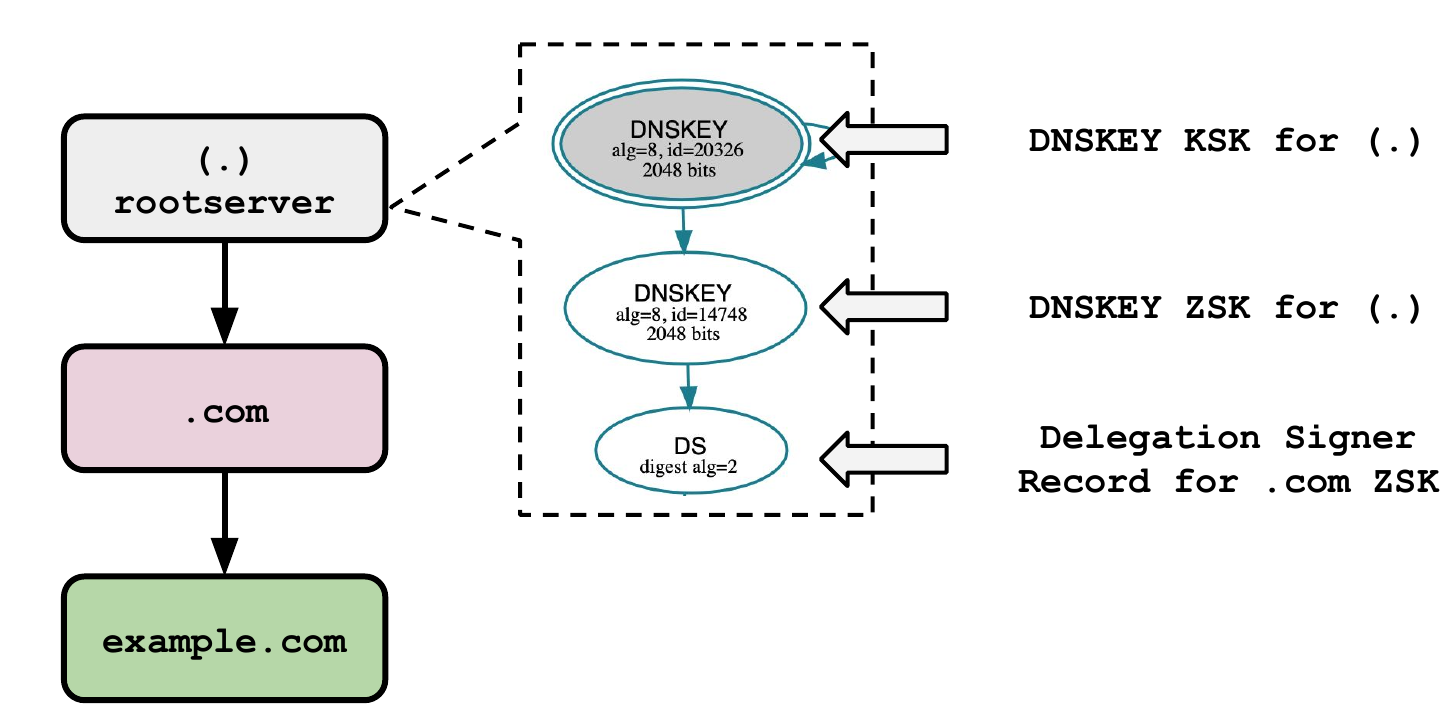
\includegraphics[scale=0.5]{../../immagini/dns_ex_1}
\end{figure}\\\\
tutti i record che vediamo firmati alla fine, guardando la situazione in DNSviz, sono set di record.
\\Vediamo poi con \texttt{dig} come è fatto un record DSNSEC, usato in questo modo: \texttt{dig +qr +dnssec @1.1.1.1 example.com A}, c'è un key tag value che è usato per calcolare la firma.
\\Abbiamo il record, ma abbiamo anche bisogno del record della chiave DNS per verificare che sia tutto corretto: \texttt{dig +qr +dnssec @1.1.1.1 example.com DNSKEY}: otteniamo 3 chiavi, di cui una però non è usata ed infatti abbiamo 2 RRKEY.
\\Ora dobbiamo validare il DS record, per essere sicuri che questo record venga dalla zona corretta, usiamo nuovamente dig: \texttt{dig +qr +dnssec @1.1.1.1 example.com DS}.
\\Nuovamente, abbiamo 6 DS record ma una singola firma perché appunto si firma l'intero set.

\section{Zone content exposure}
In legacy DNS, se facciamo una query per un dominio che non esiste otteniamo un record DNS vuoto come risposta, ma abbiamo comunque bisogno di firmarlo in DNSSEC e quindi c'è la non esistenza esplicita con i record NSEC.
\\Il record NSEC dice non esistono sottodomini fra il sottodominio x ed y, ma il problema è che siccome ogni record NSEC punta al successivo è possibile camminare su una zona finché non ha conosciuto tutta la zona, magari esponendo delle informazioni importanti.
\\È possibile nuovamente vedere questo sia con \texttt{dig} che con DSNviz.
\\Ci viene quindi in mente che i record DNS non dovrebbero essere segreti, ma anche fare il reveal di contenuti delle subzone non è il massimo.
\\Introduciamo quindi alcuni modi per evitare questo
\subsection{NSEC3}
Record type cheè una estensione di NSEC, non vengono riportati in chiaro le distanze fra i due sottodomini, ma in formato salted hashed\\ 
\begin{figure}[h!]
    \centering
    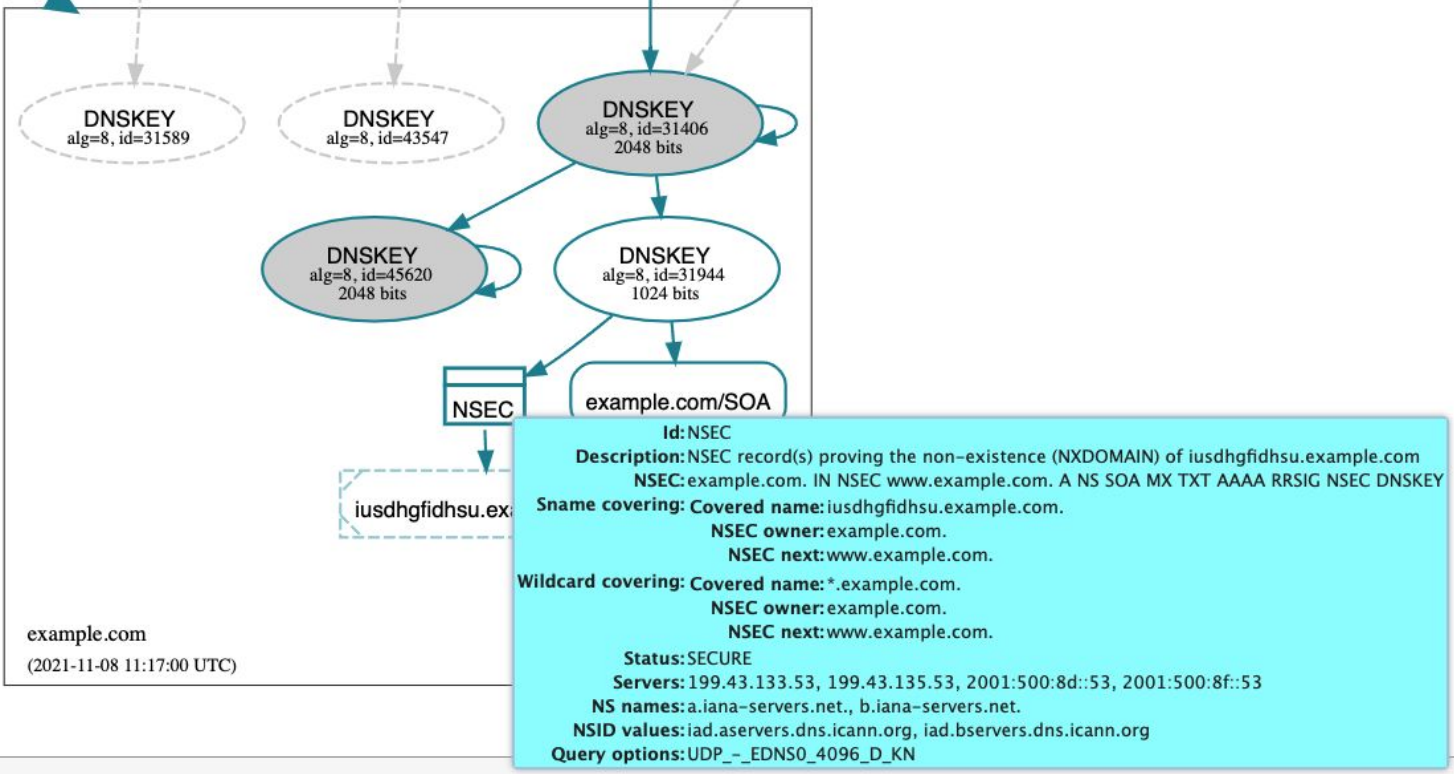
\includegraphics[scale=0.5]{../../immagini/nsec3_sh}
\end{figure}\\\\
sono salted hashed, non cifrati, quindi si può ancora tentare con degli attacchi a dizionario.
\\Si può mitigare la vulnerabilità inserendo DNSSEC white lies: mentiamo sui nomi, se richiedo per "computer.bits", non rispondiamo che non ci sono nomi fra x ed y ma usiamo dei nomi random che sono fra il nome che richiedo ed il prossimo valore reale.
\\Il problema è che per firmare questi nomi falsi va fatto on-the-fly, con RSA è abbastanza pesante, per cui  si potrebbe pensare di applicare crittografia su curve ellittiche.
\\Abbiamo comunque dei problemi: 
\begin{itemize}
	\item reflection/amplification threat: vulnerabile a reflection attack.
    \\DNSSEC lavora anche con UDP ed una risposta ad una query può contenere molteplici DNSKEY e record RRSIG.
    \\È appetibile per gli attaccanti in quanto permette di amplificare il reflection attack: se una piccola parte di richieste DNSSEC spoofate su UDP viene inviata ai nameserver, la vittima riceverà un importante traffico riflesso, conseguenza DoS.
	\item DDoS amplification: ogni volta che viene richiesto un record a DNSSEC viene anche restituita la firma associata, così come la chiave pubblica.
    \\Far si che la taglia della risposta di DNSSEC sia piccola è importante per prevenire un abuso dell'infrastruttura.
        \\ECDSA è usato pochissimo (0.01\% dei dominii) ma permette di proteggersi da:
        \begin{itemize}
            \item zone enumeration
            \item DDoS amplification
        \end{itemize}
\end{itemize}

\subsection{Cosa risolve DNSSEC e cosa No}
NDSSEC può risolvere diversi problemi, ma ci sono comunque delle cose che non si possono risolvere: (slides)\\Di sicuro, non si risolve la privacy di un client in quanto con DNS legacy i messaggi sono mandati in chiaro.\\Inoltre, DNSSEC non è deployato ovunque

\section{DNS over HTTPS o TLS}
Siccome DSNSEC non copre la privacy, abbiamo due ragioni per avere questa architettura:
\begin{itemize}
	\item privacy, così da avere le query cifrate
	\item sicurezza, in quanto gli stub resolver sono minimali ed usano solitamente query ricorsive.
    \\Non è detto che vadano a validare i record DNSSEC, quindi dobbiamo fidarci del nostro nameserver, ma se il canale di comunicazione non è protetto c'è un problema
\end{itemize}
Abbiamo quindi due soluzioni:
\begin{itemize}
	\item dns over tls vuole fornire privacy ed autenticazione per TLS.
    \\Un server che supporta DNS over TLS accetta connessioni TCP sulla 853.
    \\A questo punto, si procede con l'handshake dopo cui tutti i messaggi DNS sono mandati sul canale TLS autenticato e cifrato.
    \\Sarebbe utile mantenere attivo lo stesso canale TLS per incapsulare diverse richieste DNS
	\item con TLS over HTTPS dobbiamo poter embeddare una richiesta DNS in un pacchetto HTTP.
    \\Si può fare col metodo GET e POST:
	\begin{itemize}
		\item get: incluso in base-64 nel url
		\item in post viene messo nel corpo, il content type sarà quello corretto
	\end{itemize}
\end{itemize}
I due approcci sono simili, da un punto di vista di sicurezza della rete è meglio DoT, ma da un punto di vista della privacy è meglio DoH, qui le query sono nascoste in un traffico di rete HTTP più ampio.

\section{Lab 14: FINALE}
Laboratorio DNSSEC dove il prof si è comprato un dominio
\\Come prima cosa, occorre configurare il file di \texttt{bind}.
\\Per firmare la zona, basta lanciare un comando e si fa tutto.
\\Accade che la ZSK è anche usata per firmare il DSKEY set, il che è strano: vale anche per "example.com", verificando altri 2 domini non si trova quindi o dipende dalla configurazione oppure da qualche implementazione.

\end{document}
